\begin{frame}[t] \frametitle{LLM in contesti \emph{business}}
\framesubtitle{Riassunto delle puntate precedenti}
{\small
\onslide<1->
    \begin{minipage}[t]{\textwidth}
        \begin{itemize}[leftmargin=10pt,align=right]
            \item[\alert{\faArrowCircleRight}] Praticamente impossibile pre-addestrare un LLM (a meno che tu non sia Google, OpenAI, Mistral, Anthropic e pochissimi altri)
            \item[\alert{\faArrowCircleRight}] Utilizzare un LLM per scopi personali è un conto, adottarli in un contesto \emph{business} significa scontrarsi con problematiche di natura etica, legale ed economica
            \item[\alert{\faArrowCircleRight}] Gli LLM saranno sempre più bravi a modellare la comprensione del linguaggio$\ldots$
        \end{itemize}
        \vspace*{.5cm}
        \centering {\normalsize \textbf{\alert{\faQuestionCircleO\ $\ldots$ ma come usarli per \emph{task} specifici\\o con conoscenza che a loro manca?!}}}
    \end{minipage}
}
\end{frame}
%
\begin{frame}[t] \frametitle{\emph{Fine-tuning}}
\framesubtitle{Definizione}
{\scriptsize
\onslide<1->
    \begin{minipage}[t]{\textwidth}
        \vspace*{-.5cm}
        \begin{figure}
            \centering
            \includegraphics[width=.25\textwidth]{img/FT_1.PNG}
            \includegraphics[width=.25\textwidth]{img/FT_2.PNG}
            \includegraphics[width=.25\textwidth]{img/FT_3.PNG}
        \end{figure}
    \end{minipage}
}
\end{frame}
%
\begin{frame}[t] \frametitle{Addestramento neurale}
\framesubtitle{Approcci principali}
{\small
\onslide<1->
	\begin{itemize}[leftmargin=10pt,align=right]
		\item[\alert{\faArrowCircleRight}] \emph{Full learning}
		\begin{itemize}[leftmargin=10pt,align=right]
			\item[\alert{\faArrowCircleRight}] Creare una architettura neurale da zero$\ldots$
			\item[\alert{\faArrowCircleRight}] $\ldots$ oppure scegliere una architettura in letteratura (per i meno sadici)
			\item[\alert{\faArrowCircleRight}] Addestramento da zero (a partire da pesi e \emph{bias random})
		\end{itemize}
		\onslide<2->
		\item[\alert{\faArrowCircleRight}] \emph{Transfer learning}
		\begin{itemize}[leftmargin=10pt,align=right]
			\item[\alert{\faArrowCircleRight}] Sfruttare una rete neurale gi\'{a} addestrata su un altro insieme di dati di addestramento
			\item[\alert{\faArrowCircleRight}] Modificare solo alcuni strati (solitamente gli ultimi) per addestrare la rete per i propri scopi
		\end{itemize}
	\end{itemize}
	\onslide<3->
	{\footnotesize
		\begin{table}
			%% increase table row spacing, adjust to taste
			\renewcommand{\arraystretch}{1}
			\centering
			\begin{tabularx}{\textwidth}{Xp{2.5cm}p{2.5cm}}
				\toprule
				\textbf{\emph{Computer Vision}} & \textbf{\emph{Full learning}} & \textbf{\emph{Transfer learning}}\\
				\midrule

				\textbf{Numero dati addestramento} & $10^{3}$--$10^{6}$ & $10^{2}$\\
				\textbf{Computazione} & Intensiva (GPU) & Media (CPU--GPU)\\
				\textbf{Tempo di addestramento} & Giorni--settimane & Ore--giorni\\
				\textbf{Accuratezza del modello} & Alta & Variabile\\
				\bottomrule
			\end{tabularx}
		\end{table}
	}
}
\end{frame}
%
\begin{frame}[t] \frametitle{\emph{Fine-tuning}}
\framesubtitle{Il DNA del DL non mente$\ldots$}
{\small
\onslide<1->
    \begin{minipage}[t]{\textwidth}
        \begin{itemize}[leftmargin=10pt,align=right]
            \onslide<2->\item[\alert{\faArrowCircleRight}] ChatGPT parla del \emph{fine-tuning} per LLM come sinonimo di \emph{transfer learning}
            \onslide<3->\item[\alert{\faArrowCircleRight}] Si parla di \emph{\alert{full fine-tuning}} quando nessuno strato viene congelato
            \onslide<4->\item[\alert{\faArrowCircleRight}] Diverse tecniche per quanto riguarda il ``\emph{transfer tuning}''
            \begin{itemize}[leftmargin=10pt,align=right]
            \onslide<5->\item[\alert{\faArrowCircleRight}] \emph{\alert{M}ulti-\alert{L}evel \alert{F}ine-\alert{T}uning} (MLFT)
            \onslide<6->\item[\alert{\faArrowCircleRight}] \emph{\alert{P}arameter \alert{E}fficient \alert{F}ine-\alert{T}uning} (PEFT)
            \onslide<7->\item[\alert{\faArrowCircleRight}] \alert{\emph{\alert{Lo}w-\alert{R}ank \alert{A}daptation} (LoRA)}
            \onslide<8->\item[\alert{\faArrowCircleRight}] Adapter Training
            \onslide<9->\item[\alert{\faArrowCircleRight}] $\ldots$
            \end{itemize}
        \end{itemize}
    \end{minipage}
}
\end{frame}
%
\begin{frame}[t] \frametitle{\emph{Quantization}}
\framesubtitle{Ottimizzazione per \emph{full fine-tuning}}
{\scriptsize
\onslide<1->
    \begin{minipage}[t]{\textwidth}
        \vspace*{-.5cm}
        \begin{itemize}[leftmargin=10pt,align=right]
            \onslide<1->\item[\alert{\faArrowCircleRight}] Possibile eseguire \emph{full fine-tuning} su LLM pre-addestrate di dimensioni ``contenute''$\ldots$
            \onslide<2->\item[\alert{\faArrowCircleRight}] $\ldots$ facendo attenzione a non esagerare$\ldots$
            \onslide<3->\item[\alert{\faArrowCircleRight}] $\ldots$ e possibilmente, \alert{ottimizzando il processo} decidendo la precisione dei parametri del modello (ovvero, \emph{quantizzandolo})
        \end{itemize}
    \end{minipage}
    \begin{minipage}[t]{\textwidth}
        \vspace*{.2cm}
            \begin{figure}
                \centering
                \includegraphics[width=.7\textwidth]{img/quantization-no-bg.png}
                {\tiny\\Quantizzazione\\\vspace*{-1pt}\textit{\textcopyright Cerebras}}
            \end{figure}
    \end{minipage}
    \begin{minipage}[t]{\textwidth}
        \vspace*{.2cm}
        \begin{itemize}[leftmargin=10pt,align=right]
            \onslide<4->\item[\alert{\faArrowCircleRight}] Quantizzazione a \texttt{float16} e \texttt{bfloat16} usati maggiormente per addestramento
            \item[\alert{\faArrowCircleRight}] \texttt{bfloat16} generalmente preferito a \texttt{float16}
            \onslide<5->\item[\alert{\faArrowCircleRight}] Addestramento a \texttt{float32} riservato alle \emph{big companies}
            \onslide<6->\item[\alert{\faArrowCircleRight}] Quantizzazioni inferiori disponibili (\texttt{int8}, \texttt{int4}), ma consigliate solo per inferenza
        \end{itemize}
    \end{minipage}
}
\end{frame}
%
\begin{frame}[t] \frametitle{\emph{Quantization}}
\framesubtitle{Visione concettuale}
{\scriptsize
\onslide<1->
    \begin{minipage}[t]{\textwidth}
        \vspace*{-.3cm}
        \begin{figure}
            \centering
            \includegraphics[width=.8\textwidth]{img/quantization_concept_no_bg.png}
            {\tiny\\Quantizzazione\\\vspace*{-1pt}\textit{\textcopyright jeremy jouvance@GoPenAI}}
        \end{figure}
    \end{minipage}
    \\\vspace*{.3cm}
    \begin{minipage}[t]{\textwidth}
        \begin{itemize}[leftmargin=10pt,align=right]
            \onslide<2->\item[\alert{\faArrowCircleRight}] A favore del peso del modello in memoria e ai tempi di addestramento$\ldots$
            \onslide<3->\item[\alert{\faArrowCircleRight}] $\ldots$ a scapito dell'accuratezza in fase di inferenza
            \onslide<4->\item[\alert{\faArrowCircleRight}]\emph{Tradeoff} fra risorse e prestazioni dettato anche dalla strategia adottata
            \begin{itemize}[leftmargin=10pt,align=right]
                \onslide<5->\item[\alert{\faArrowCircleRight}] Quantizzazione terminato il processo di addestramento (\alert{P}ost \alert{T}raining \alert{Q}uantization -- PTQ)
                \onslide<6->\item[\alert{\faArrowCircleRight}] Quantizzazione durante l'addestramento (\emph{\alert{Q}uantization-\alert{A}ware \alert{T}raining (QAT)})
            \end{itemize}
        \end{itemize}
    \end{minipage}
}
\end{frame}
%
\begin{frame}[t] \frametitle{LoRA}
	{\scriptsize
		\onslide<1->
            \framesubtitle{Rivoluzione nel mondo dell'addestramento LLM}
            \vspace*{-.5cm}
             \begin{minipage}[t]{\textwidth}
             	\begin{figure}[ht]
                    \centering
                    \includegraphics[width=\textwidth]{img/AI-timeline-2021.png}
                \end{figure}
            \end{minipage}
            \\\vspace*{.3cm}
	    	\begin{minipage}[t]{.35\textwidth}
                \begin{itemize}[leftmargin=10pt,align=right]
						\onslide<2->\item[\alert{\faArrowCircleRight}] Variazione di PEFT
						\onslide<3->\item[\alert{\faArrowCircleRight}] Si riaddestrano solo un sottoinsieme $\Delta W$ di parametri esplicitamente selezionati (una sorta di \emph{transfer learning})$\ldots$
						\onslide<4->\item[\alert{\faArrowCircleRight}] $\ldots$ mantenendo fissi tutti gli altri $W$
                        \onslide<5->\item[\alert{\faArrowCircleRight}] Fissato un parametro $r$ (\alert{rango}), LoRA approssima $\Delta W$ come prodotto scalare di due matrici più piccole
                \end{itemize}
	    	\end{minipage}
    \hfill
    \onslide<1->
        \begin{minipage}[t]{.60\textwidth}
            \begin{figure}[ht]
                \centering
                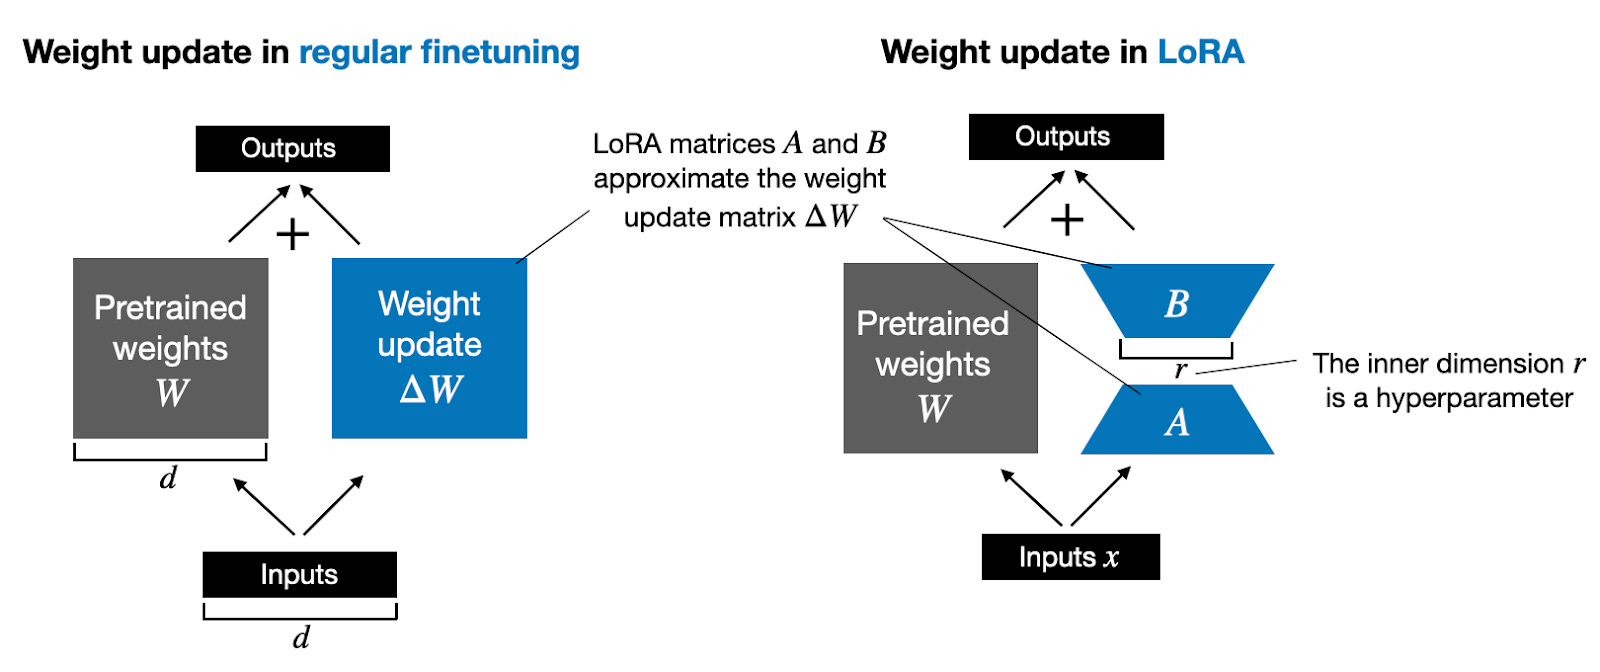
\includegraphics[width=\textwidth]{img/LoRA.png}
                {\tiny\\LoRA\\\vspace*{-1pt}\textit{\textcopyright Sebastian Raschka@Ahead of AI}}
            \end{figure}
        \end{minipage}
	}
\end{frame}
%
\begin{frame}[t] \frametitle{LoRA}
\framesubtitle{Principi algebrici}
{\tiny
    \begin{minipage}[t]{\textwidth}
        \vspace*{-.5cm}
        \begin{block}{Prodotto scalare}
            Il \emph{prodotto scalare} di matrice ($n \times r$) $A = \begin{bmatrix}
                                                                            a_{11} & a_{12} & \ldots & a_{1r}\\
                                                                            \vdots & \vdots & \vdots & \vdots\\
                                                                            a_{n1} & a_{n2} & \ldots & a_{nr}\\
            \end{bmatrix}$ e matrice ($r \times m$)
            $B = \begin{bmatrix}
                     b_{11} & b_{12} & \ldots & b_{1m}\\
                     \vdots & \vdots & \vdots & \vdots\\
                     b_{r1} & b_{r2} & \ldots & b_{rm}\\
            \end{bmatrix}$ é la matrice ($n \times m$)
            \begin{displaymath}
                A\cdot B =
                \begin{bmatrix}
                    a_{11}*b_{11} + \ldots + a_{1r}*b_{r1}& \ldots & a_{11}*b_{1m} + \ldots + a_{1r}*b_{rm}\\
                    \vdots & \vdots & \vdots\\
                    a_{n1}*b_{11} + \ldots + a_{nr}*b_{r1}& \ldots & a_{n1}*b_{1m} + \ldots + a_{nr}*b_{rm}\\
                \end{bmatrix}
            \end{displaymath}
        \end{block}
    \end{minipage}
    \begin{minipage}[t]{\textwidth}
        \vspace*{.5cm}
        {\small
        \begin{itemize}[leftmargin=10pt,align=right]
            \onslide<2->\item[\alert{\faArrowCircleRight}] In pratica, fissato $r$, LoRA computa $A$ e $B$ tale per cui $\Delta W = A\cdot B$
            \onslide<3->\item[\alert{\faArrowCircleRight}] Ma perché é così potente?!
        \end{itemize}
        }
    \end{minipage}
}
\end{frame}
%
\begin{frame}[t] \frametitle{LoRA}
\framesubtitle{Principi algebrici}
{\small
    \begin{minipage}[t]{\textwidth}
        \vspace*{-.5cm}
        \begin{block}{Esempio LoRA}
            \[
                \Delta W =
                \begin{bmatrix}
                5 & 1 & -1 & 3 & 4\\
                15 & 3 & -3 & 9 & 12\\
                35 & 7 & -7 & 21 & 28\\
                -20 & -4 & 4 & -12 & -16\\
                10 & 2 & -2 & 6 & 8\\
                \end{bmatrix} \xLongrightarrow[]{\text{LoRA($r=1$)}}
                A =
                    \begin{bmatrix}
                        1 \\
                        3 \\
                        7 \\
                        -4\\
                        2
                    \end{bmatrix},\ B=
                    \begin{bmatrix}
                        5 & 1 & -1 & 3 & 4
                    \end{bmatrix}
            \]
        \end{block}
    \end{minipage}
    \begin{minipage}[t]{\textwidth}
        \vspace*{.5cm}
        {\small
            \begin{itemize}[leftmargin=10pt,align=right]
                \onslide<2->\item[\alert{\faArrowCircleRight}] Numero parametri da salvare?
                \begin{itemize}[leftmargin=10pt,align=right]
                    \onslide<3->\item[\alert{\faArrowCircleRight}] $\Delta W$: 25
                    \item[\alert{\faArrowCircleRight}] $A$ e $B$ (totale): 10
                    \onslide<4->\item[\alert{\faArrowCircleRight}] Risparmio spazio: \alert{40\%}
                \end{itemize}
                \onslide<5->\item[\alert{\faArrowCircleRight}] La \emph{backpropagation} opera direttamente sulle rappresentazioni di $A$ e $B$!
                \onslide<6->\item[\alert{\faExclamationTriangle}] Metodo di \alert{approssimazione}, quindi a scapito della \emph{accuracy} del modello
            \end{itemize}
        }
    \end{minipage}
}
\end{frame}
%
\begin{frame}[t] \frametitle{QLoRA}
{\small
\onslide<1->
\framesubtitle{Cosa sarà mai$\ldots$?}
\vspace*{-.5cm}
    \begin{minipage}[t]{\textwidth}
        \begin{figure}[ht]
            \centering
            \includegraphics[width=\textwidth]{img/AI-timeline-2023.png}
        \end{figure}
    \end{minipage}
    \\\vspace*{.3cm}
    \begin{minipage}[t]{\textwidth}
        \begin{itemize}[leftmargin=10pt,align=right]
            \onslide<2->\item[\alert{\faArrowCircleRight}] Decomposizione LoRA + \emph{Quantization}$\ldots$
            \onslide<3->\item[\alert{\faArrowCircleRight}] $\ldots$ tutto qui.
        \end{itemize}
    \end{minipage}
}
\end{frame}
%